\subsubsection{UCA 6 - Tracciamento movimento presso un'organizzazione e i luoghi all'interno di essa}%kite level

%\begin{figure}[h]
%	\centering
%	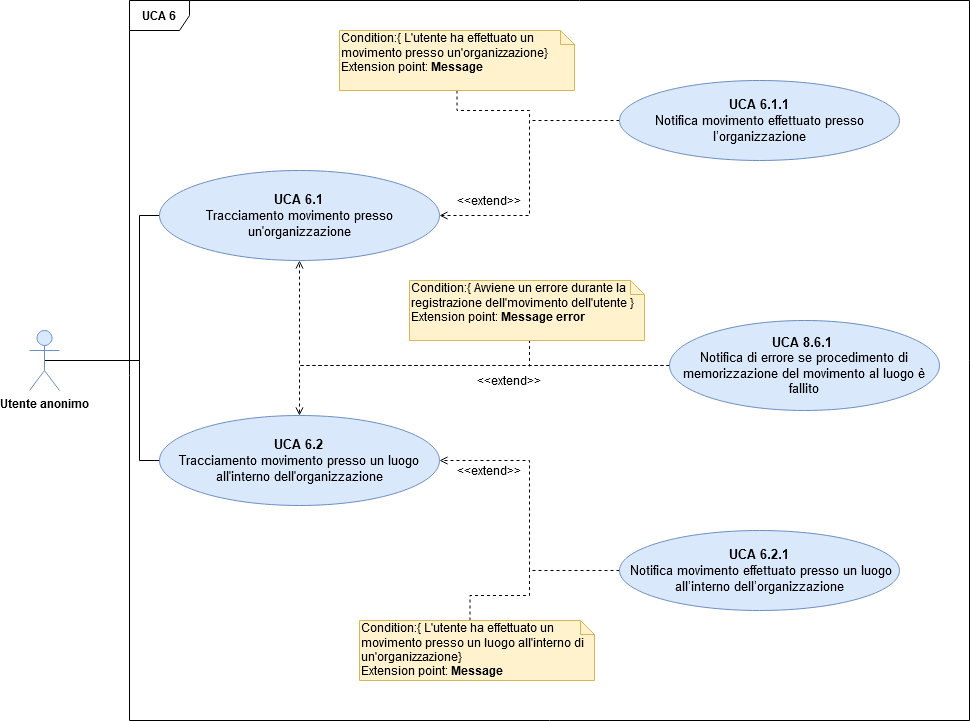
\includegraphics[scale=0.3, center]{Sezioni/UseCase/Immagini/UCA6.png}
%	\caption{\glo{Tracciamento} posizione in un luogo di un'\glo{organizzazione}}
%\end{figure}

\begin{itemize}
	\item \textbf{Attori primari:} Utente anonimo, Utente riconosciuto
	\item \textbf{Attori secondari:} Servizi/o di localizzazione (\glo{GPS}, rete cellulare)
	\item \textbf{Precondizione:} L'utente sta per effettuare un \glo{movimento} in un'\glo{organizzazione} o in un luogo all'interno di essa.
	\item \textbf{Postcondizione:} L'utente ha effettuato un \glo{movimento} presso l'\glo{organizzazione} o in un luogo all'interno di essa e ne viene notificato l'avvenimento. %e vengono salvate alcune cose (memorizzazione timestamp, ecc)? 
	\item \textbf{Scenario principale:} L'utente si trova nei pressi o all'interno di un'\glo{organizzazione} o di un suo luogo e sta per effettuare un \glo{movimento}. L'utente riceve una notifica una volta effettuato il movimento. %Viene salvato l'orario di entrata ed uscita dall'\glo{organizzazione} e il tempo trascorso all'interno dell'\glo{organizzazione}. L'utente riceve inoltre una notifica per l'entrata e l'uscita dall'\glo{organizzazione}.
\end{itemize}

\subsubsection{UCA 6.1 - Tracciamento movimento presso un'organizzazione}
\begin{itemize}
	\item \textbf{Attori primari:} Utente anonimo, Utente riconosciuto
	\item \textbf{Attori secondari:} Servizi/o di localizzazione (\glo{GPS}, rete cellulare)
	\item \textbf{Precondizione:} L'utente sta per effettuare un \glo{movimento} in un'\glo{organizzazione}.
	\item \textbf{Postcondizione:} L'utente ha effettuato un \glo{movimento} presso l'\glo{organizzazione} e ne viene notificato l'avvenimento.
	\item \textbf{Scenario principale:} L'utente si trova nei pressi o all'interno di un'\glo{organizzazione} e sta per effettuare un \glo{movimento}. L'utente riceve una notifica una volta effettuato il movimento.
	%\item \textbf{Scenario alternativo:} .
	\item \textbf{Flusso di eventi:}
	\begin{enumerate}
		\item L'utente effettua un movimento nei pressi di un'\glo{organizzazione};
		\item L'utente riceve una notifica del movimento effettuato [6.1.1].
	\end{enumerate}
	%\item \textbf{Estensioni:}
	%\begin{itemize}
		%\item UCA 8.6.1 - Notifica di errore se procedimento di memorizzazione del movimento al luogo è fallito.
	%\end{itemize}
\end{itemize}

\subsubsection{UCA 6.1.1 - Notifica movimento effettuato presso l'organizzazione}
\begin{itemize}
	\item \textbf{Attori primari:} Utente anonimo, Utente riconosciuto
	\item \textbf{Precondizione:} L'utente ha effettuato un \glo{movimento} presso l'\glo{organizzazione}.
	\item \textbf{Postcondizione:} L'utente riceve una notifica del movimento effettuato.
	\item \textbf{Scenario principale:} L'utente una volta effettuato il movimento riceve una notifica.	
\end{itemize}

\subsubsection{UCA 6.2 - Tracciamento movimento presso un luogo all'interno dell'organizzazione}
\begin{itemize}
	\item \textbf{Attori primari:} Utente anonimo, Utente riconosciuto
	\item \textbf{Attori secondari:} Servizi/o di localizzazione (\glo{GPS}, rete cellulare).
	\item \textbf{Precondizione:} L'utente autenticato sta per effettuare un \glo{movimento} in un luogo all'interno di un'\glo{organizzazione}.
	\item \textbf{Postcondizione:} L'utente ha effettuato un \glo{movimento} presso un luogo all'interno di un'\glo{organizzazione} e ne viene notificato l'avvenimento.
	\item \textbf{Scenario principale:} L'utente sta per effettuare un movimento in un luogo all'interno di un'\glo{organizzazione}. L'utente riceve una notifica una volta effettuato il movimento.
	%\item \textbf{Scenario alternativo:} .
	\item \textbf{Flusso di eventi:}
	\begin{enumerate}
		\item L'utente effettua un movimento in un luogo all'interno di un'\glo{organizzazione};
		\item L'utente riceve una notifica del movimento effettuato [6.2.1].
	\end{enumerate}
	%\item \textbf{Estensioni:}
	%\begin{itemize}
		%\item UCA 8.6.1 - Notifica di errore se procedimento di memorizzazione del movimento al luogo è fallito.
	%\end{itemize}
\end{itemize}

\subsubsection{UCA 6.2.1 - Notifica movimento effettuato presso un luogo all'interno dell'organizzazione}
\begin{itemize}
	\item \textbf{Attori primari:} Utente anonimo, Utente riconosciuto
	\item \textbf{Attori secondari:} Servizi/o di localizzazione (\glo{GPS}, rete cellulare).
	\item \textbf{Precondizione:} L'utente ha effettuato un \glo{movimento} presso un luogo all'interno dell'\glo{organizzazione}.
	\item \textbf{Postcondizione:} L'utente riceve una notifica del movimento effettuato.
	\item \textbf{Scenario principale:} L'utente una volta effettuato il movimento riceve una notifica.
\end{itemize}














